\documentclass[11pt, a4paper]{report}

% ========== Common Packages ==========
\usepackage{fontspec}
\usepackage{kotex}
\usepackage{amsmath, amssymb, amsthm}
\usepackage{mathtools}
\usepackage{bm}
\usepackage{graphicx}
\usepackage{booktabs}
\usepackage{array}
\usepackage{tabularx}
\usepackage{longtable}
\usepackage{hyperref}
\usepackage{cleveref}
\usepackage{geometry}
\usepackage{fancyhdr}
\usepackage{titlesec}
\usepackage{enumitem}
\usepackage{xcolor}
\usepackage{tcolorbox}
\usepackage{algorithm}
\usepackage{algorithmic}
\usepackage{tikz}
\usetikzlibrary{arrows.meta, positioning, calc, decorations.pathreplacing, shapes.geometric, fit, patterns, angles, quotes, trees}
\usepackage{pgfplots}
\pgfplotsset{compat=1.18}
\usepackage{caption}
\usepackage{subcaption}
\usepackage{float}

\geometry{margin=2.5cm, top=3cm, bottom=3cm}

\usepackage{multirow}
\usepackage{siunitx}
% ========== Colors ==========
% Common
\definecolor{defblue}{RGB}{30, 80, 150}
\definecolor{thmgreen}{RGB}{20, 110, 60}
\definecolor{noteorange}{RGB}{200, 100, 0}
\definecolor{lightblue}{RGB}{230, 240, 255}
\definecolor{lightgreen}{RGB}{230, 255, 235}
\definecolor{lightorange}{RGB}{255, 245, 230}
\definecolor{lightgray}{RGB}{245, 245, 245}
% Extended
\definecolor{lightred}{RGB}{255, 235, 235}
\definecolor{darkred}{RGB}{180, 30, 30}
\definecolor{biogreen}{RGB}{10, 130, 80}
\definecolor{cvpurple}{RGB}{100, 40, 150}
\definecolor{injuryred}{RGB}{200, 40, 40}
\definecolor{codegray}{RGB}{240, 240, 245}
\definecolor{pipeblue}{RGB}{25, 100, 180}
\definecolor{constraintred}{RGB}{200, 50, 50}
\definecolor{termblack}{RGB}{30, 30, 30}
\definecolor{goldcolor}{RGB}{180, 140, 20}

% ========== Theorem-like environments ==========
\theoremstyle{definition}
\newtheorem{definition}{Definition}[chapter]
\newtheorem{example}{Example}[chapter]

\theoremstyle{plain}
\newtheorem{theorem}{Theorem}[chapter]
\newtheorem{proposition}{Proposition}[chapter]

\theoremstyle{remark}
\newtheorem{remark}{Remark}[chapter]

% ========== tcolorbox environments ==========
% --- Common (all parts) ---
\newtcolorbox{keyidea}[1][]{
  colback=lightblue,
  colframe=defblue,
  fonttitle=\bfseries,
  title={Key Idea},
  #1
}

\newtcolorbox{importantnote}[1][]{
  colback=lightorange,
  colframe=noteorange,
  fonttitle=\bfseries,
  title={Important},
  #1
}

\newtcolorbox{summary}[1][]{
  colback=lightgreen,
  colframe=thmgreen,
  fonttitle=\bfseries,
  title={Summary},
  #1
}

% --- Warning/Error ---
\newtcolorbox{warningbox}[1][]{
  colback=lightred,
  colframe=darkred,
  fonttitle=\bfseries,
  title={Warning},
  #1
}

% --- Domain: Biomechanics & Clinical ---
\newtcolorbox{clinicalnote}[1][]{
  colback=lightred,
  colframe=darkred,
  fonttitle=\bfseries,
  title={Clinical Note},
  #1
}

\newtcolorbox{biomechbox}[1][]{
  colback=lightgreen,
  colframe=biogreen,
  fonttitle=\bfseries,
  title={Biomechanics},
  #1
}

\newtcolorbox{injurybox}[1][]{
  colback={injuryred!8},
  colframe=injuryred,
  fonttitle=\bfseries,
  title={Injury Risk},
  #1
}

% --- Domain: Computer Vision ---
\newtcolorbox{cvbox}[1][]{
  colback={cvpurple!5},
  colframe=cvpurple,
  fonttitle=\bfseries,
  title={Computer Vision},
  #1
}

% --- Pipeline & Setup ---
\newtcolorbox{setupbox}[1][]{
  colback=lightgray,
  colframe=gray!60,
  fonttitle=\bfseries,
  title={Setup},
  #1
}

\newtcolorbox{pipelinebox}[1][]{
  colback=pipeblue!5,
  colframe=pipeblue,
  fonttitle=\bfseries,
  title={Pipeline Step},
  #1
}

\newtcolorbox{codebox}[1][]{
  colback=codegray,
  colframe=gray!70,
  fonttitle=\bfseries\ttfamily,
  title={Code},
  #1
}

\newtcolorbox{termbox}[1][]{
  colback=termblack!5,
  colframe=termblack!60,
  fonttitle=\bfseries\ttfamily,
  title={Terminal},
  #1
}

% --- Research ---
\newtcolorbox{hypothesis}[1][]{
  colback=goldcolor!8,
  colframe=goldcolor,
  fonttitle=\bfseries,
  title={Hypothesis},
  #1
}

\newtcolorbox{resultbox}[1][]{
  colback=thmgreen!8,
  colframe=thmgreen,
  fonttitle=\bfseries,
  title={Expected Result},
  #1
}

% --- Constraints & Solutions ---
\newtcolorbox{constraintbox}[1][]{
  colback=constraintred!8,
  colframe=constraintred,
  fonttitle=\bfseries,
  title={Constraint},
  #1
}

\newtcolorbox{solutionbox}[1][]{
  colback=thmgreen!8,
  colframe=thmgreen,
  fonttitle=\bfseries,
  title={Solution},
  #1
}

\newtcolorbox{databox}[1][]{
  colback=pipeblue!5,
  colframe=pipeblue,
  fonttitle=\bfseries,
  title={Data Spec},
  #1
}

% --- Progress/Status ---
\newtcolorbox{successbox}[1][]{
  colback=lightgreen,
  colframe=thmgreen,
  fonttitle=\bfseries,
  title={Success},
  #1
}

\newtcolorbox{nextbox}[1][]{
  colback=lightorange,
  colframe=noteorange,
  fonttitle=\bfseries,
  title={Next Step},
  #1
}

% --- Fitting guide ---
\newtcolorbox{failbox}[1][]{
  colback=lightred,
  colframe=darkred,
  fonttitle=\bfseries,
  title={Failure Pattern},
  #1
}

\newtcolorbox{fixbox}[1][]{
  colback=lightgreen,
  colframe=thmgreen,
  fonttitle=\bfseries,
  title={Fix},
  #1
}

\newtcolorbox{lessonbox}[1][]{
  colback=lightorange,
  colframe=noteorange,
  fonttitle=\bfseries,
  title={Lesson Learned},
  #1
}

% --- Specification ---
\newtcolorbox{specbox}[1][]{
  colback=cvpurple!5,
  colframe=cvpurple,
  fonttitle=\bfseries,
  title={Specification},
  #1
}

\newtcolorbox{checklistbox}[1][]{
  colback=lightgreen,
  colframe=biogreen,
  fonttitle=\bfseries,
  title={Checklist},
  #1
}

% ========== Custom math commands ==========
% Vectors (lowercase)
\newcommand{\vx}{\mathbf{x}}
\newcommand{\vd}{\mathbf{d}}
\newcommand{\vo}{\mathbf{o}}
\newcommand{\vc}{\mathbf{c}}
\newcommand{\vr}{\mathbf{r}}
\newcommand{\vp}{\mathbf{p}}
\newcommand{\vv}{\mathbf{v}}
\newcommand{\vn}{\mathbf{n}}
\newcommand{\vu}{\mathbf{u}}
\newcommand{\vt}{\mathbf{t}}
\newcommand{\ve}{\mathbf{e}}
\newcommand{\vq}{\mathbf{q}}
% Vectors (uppercase)
\newcommand{\vF}{\mathbf{F}}
\newcommand{\vM}{\mathbf{M}}
\newcommand{\va}{\mathbf{a}}
\newcommand{\vg}{\mathbf{g}}
\newcommand{\vX}{\mathbf{X}}
% Bold Greek
\newcommand{\vmu}{\bm{\mu}}
\newcommand{\vbeta}{\bm{\beta}}
\newcommand{\vtheta}{\bm{\theta}}
\newcommand{\vpsi}{\bm{\psi}}
% Matrices
\newcommand{\mSigma}{\bm{\Sigma}}
\newcommand{\mR}{\mathbf{R}}
\newcommand{\mS}{\mathbf{S}}
\newcommand{\mW}{\mathbf{W}}
\newcommand{\mJ}{\mathbf{J}}
\newcommand{\mG}{\mathbf{G}}
\newcommand{\mT}{\mathbf{T}}
\newcommand{\mI}{\mathbf{I}}
\newcommand{\mB}{\mathbf{B}}
\newcommand{\mK}{\mathbf{K}}
\newcommand{\mP}{\mathbf{P}}
\newcommand{\mF}{\mathbf{F}}
\newcommand{\mE}{\mathbf{E}}
\newcommand{\mA}{\mathbf{A}}
\newcommand{\mH}{\mathbf{H}}
% Sets and groups
\newcommand{\RR}{\mathbb{R}}
\newcommand{\SO}{\mathrm{SO}}
% Units
\newcommand{\degps}{\,\text{deg/s}}
\newcommand{\Nm}{\ensuremath{\,\text{N}\cdot\text{m}}}
\newcommand{\BW}{\,\text{BW}}

% ========== Header/Footer ==========
\pagestyle{fancy}
\fancyhf{}
\fancyhead[L]{\leftmark}
\fancyhead[R]{\thepage}
\renewcommand{\headrulewidth}{0.4pt}

% ========== Title formatting ==========
\titleformat{\chapter}[display]
  {\normalfont\huge\bfseries\color{defblue}}
  {\chaptertitlename\ \thechapter}{20pt}{\Huge}

\titleformat{\section}
  {\normalfont\Large\bfseries\color{defblue!80!black}}
  {\thesection}{1em}{}

\titleformat{\subsection}
  {\normalfont\large\bfseries\color{defblue!60!black}}
  {\thesubsection}{1em}{}


\begin{document}

\begin{titlepage}
\centering
\vspace*{1.5cm}
{\Large\color{gray} Experiment Log Day 2}
\vspace{0.5cm}

{\Huge\bfseries\color{defblue} 2026년 4월 12--13일\\[0.3cm]
SMPL 피팅 $\rightarrow$ U-HMR 성공}

\vspace{1cm}

{\LARGE\color{defblue!70!black} SMPLest-X 단일뷰 $\rightarrow$ U-HMR 다시점\\
SMPL 메시 복원 파이프라인 실험 기록}

\vspace{2cm}
{\large 2026년 4월 13일}
\end{titlepage}

\tableofcontents
\newpage


% ====================================================================
\chapter{실험 흐름 요약}
% ====================================================================

\begin{table}[H]
\centering
\caption{시도한 방법들과 결과}
\renewcommand{\arraystretch}{1.4}
\small
\begin{tabular}{c p{5cm} p{3cm} c}
\toprule
\textbf{\#} & \textbf{방법} & \textbf{결과} & \textbf{상태} \\
\midrule
1 & EasyMocap (삼각측량$\rightarrow$3D$\rightarrow$SMPL) & MPJPE 1384mm & 실패 \\
2 & 직접 3D SMPL 피팅 & MPJPE 241mm & 부분 성공 \\
3 & 2D Reproj 배치 피팅 (T-pose init) & mean 50px, 3D 482mm & 부분 성공 \\
4 & ReFit (단일뷰 regression) & 후면 각도 실패 & 실패 \\
5 & SMPLest-X (단일뷰, 0.69B) & 시각적으로 양호 & 성공 \\
6 & SMPLest-X + smoothing & 떨림 감소 & 성공 \\
7 & 배치 피팅 (SMPLest-X init) & 좌표계 불일치 & 실패 \\
\textbf{8} & \textbf{U-HMR (다시점 fusion)} & \textbf{4뷰 메시 복원 성공} & \textbf{성공} \\
\bottomrule
\end{tabular}
\end{table}


% ====================================================================
\chapter{SMPLest-X 실험}
% ====================================================================

\section{접근: SAM bbox + 원본 이미지 크롭}

마스킹 이미지에서 투수의 bbox만 추출하고, 원본 이미지를 해당 bbox로 크롭하여 SMPLest-X에 입력.

\begin{itemize}[leftmargin=*]
  \item SAM mask $\rightarrow$ 투수 실루엣의 bbox 추출 (프레임별 동적)
  \item 원본 이미지에서 해당 bbox로 크롭 (자연 배경 유지)
  \item YOLO 검출 건너뛰기 $\rightarrow$ 다른 사람 잡을 위험 제거
\end{itemize}

\subsection{마스킹 vs 크롭 실험}

\begin{table}[H]
\centering
\caption{입력 이미지 방식별 SMPLest-X focal 추정 비교}
\renewcommand{\arraystretch}{1.3}
\begin{tabular}{l c c}
\toprule
\textbf{입력 방식} & \textbf{추정 focal} & \textbf{결과} \\
\midrule
마스킹 이미지 (검은 배경) & 11,808 & depth 비정상, 움직임 없음 \\
마스킹+크롭 (검은 배경) & 11,877 & 동일 문제 \\
마스킹+크롭 (회색 배경) & 12,529 & 동일 문제 \\
\textbf{원본 크롭 (자연 배경)} & \textbf{11,808} & \textbf{정상 작동} \\
SAM bbox + 원본 크롭 & 11,811 & 정상 작동 \\
\bottomrule
\end{tabular}
\end{table}

\begin{keyidea}
focal 값 자체는 모두 $\sim$11,800으로 동일. SMPLest-X의 focal은 내부적으로 고정.
\textbf{자연 배경이 있어야 depth context를 제대로 이해}하여 포즈 추정이 정확해짐.
마스킹 배경(검은색/회색)에서는 depth 단서가 사라져 포즈가 부정확.
\end{keyidea}

\subsection{결과: cam3 1000프레임}

\begin{itemize}[leftmargin=*]
  \item 처리 시간: 1000프레임 / 3.5분 (A100, 4.5 fps)
  \item SAM bbox가 프레임별 동적으로 투수 추적
  \item 포즈가 실제 투구 동작과 대체로 일치 (wind-up, stride)
  \item 문제: 프레임 간 \textbf{떨림 (jittering)} --- 단일뷰 독립 추론의 한계
\end{itemize}

\subsection{Temporal Smoothing}

Savitzky-Golay 필터 (window=15, polynomial=3)를 10,475개 정점 $\times$ 3좌표에 적용.
\begin{itemize}[leftmargin=*]
  \item 떨림이 감소했으나 완전히 해결되지는 않음
  \item 근본 원인: 단일뷰 regression은 프레임 간 일관성을 보장하지 않음
\end{itemize}


% ====================================================================
\chapter{U-HMR 실험}
% ====================================================================

\section{U-HMR이란}

\textbf{U-HMR} (Unified Human Mesh Recovery from Arbitrary Multi-view Images):
\begin{itemize}[leftmargin=*]
  \item 임의 개수의 카메라 뷰를 동시 입력하여 SMPL 메시 복원
  \item Camera and Body Decoupling (CBD): 카메라 포즈와 인체 메시를 분리 추정
  \item Arbitrary View Fusion (AVF): Transformer decoder로 다시점 정보 융합
  \item Human3.6M에서 다시점 MPJPE 31.0mm (단일뷰 43.3mm 대비 28\% 개선)
\end{itemize}

\section{설치 및 설정}

\begin{enumerate}[leftmargin=*]
  \item 코드: \texttt{github.com/XiaobenLi00/U-HMR}
  \item Pretrained weights: OneDrive에서 \texttt{vit\_pos\_trans\_encoder\_token} 다운로드 (8.2GB)
  \item SMPL 모델: v1.1.0 (faces=13,776) --- 서버에 업로드 완료
  \item 추가 파일: \texttt{SMPL\_to\_J19.pkl} (체크포인트에서 추출), \texttt{smpl\_mean\_params.npz}
  \item 수정: \texttt{strict=False}로 모델 로드 (discriminator 미사용)
\end{enumerate}

\section{결과: 4대 카메라 다시점 추론}

4대 카메라 (cam3, cam5, cam6, cam7)의 크롭 이미지를 동시 입력하여 SMPL 메시 복원 성공.

\begin{figure}[H]
\centering
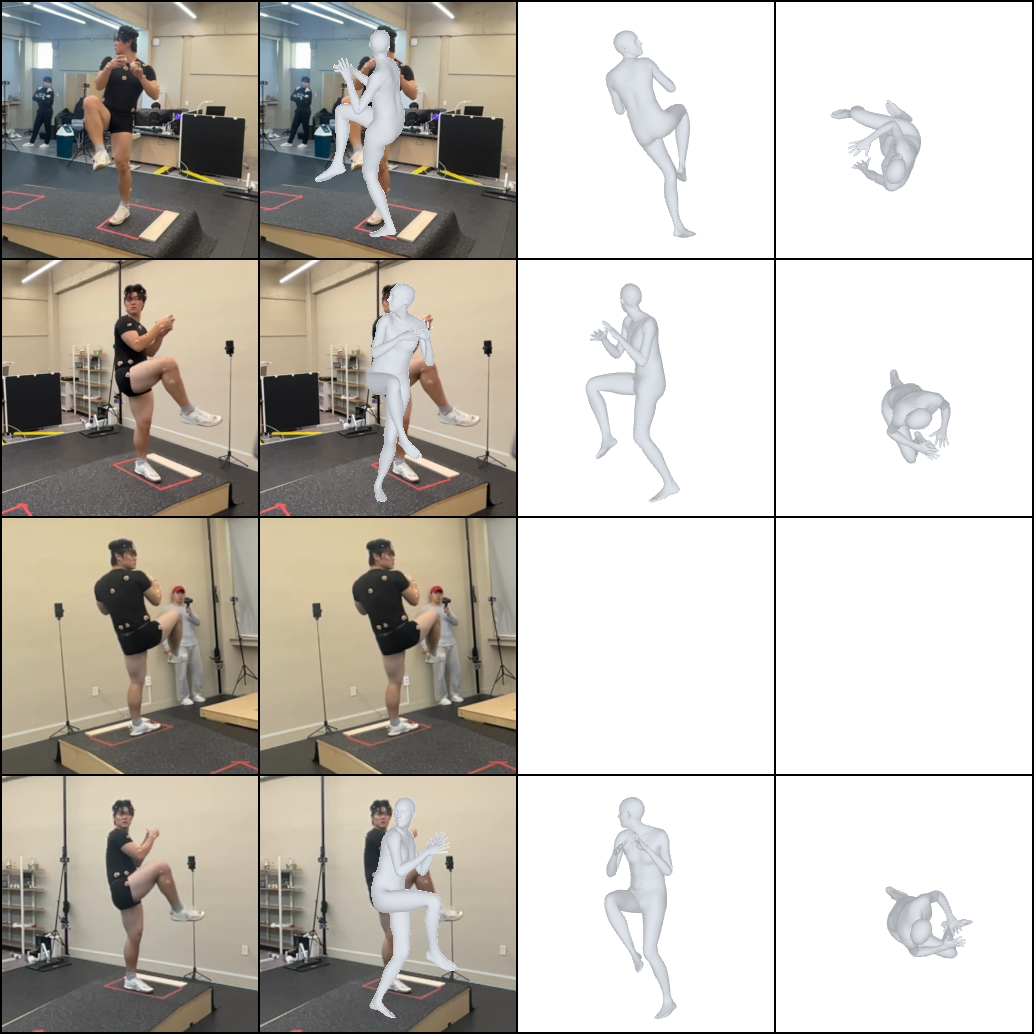
\includegraphics[width=0.7\textwidth]{data/uhmr_result/mesh_vis1.png}
\caption{U-HMR 다시점 결과: 4개 뷰의 원본 이미지(좌), SMPL 메시 오버레이(중), 3D 메시 렌더링(우). 투수의 wind-up 포즈가 정확히 복원됨.}
\end{figure}

\begin{figure}[H]
\centering
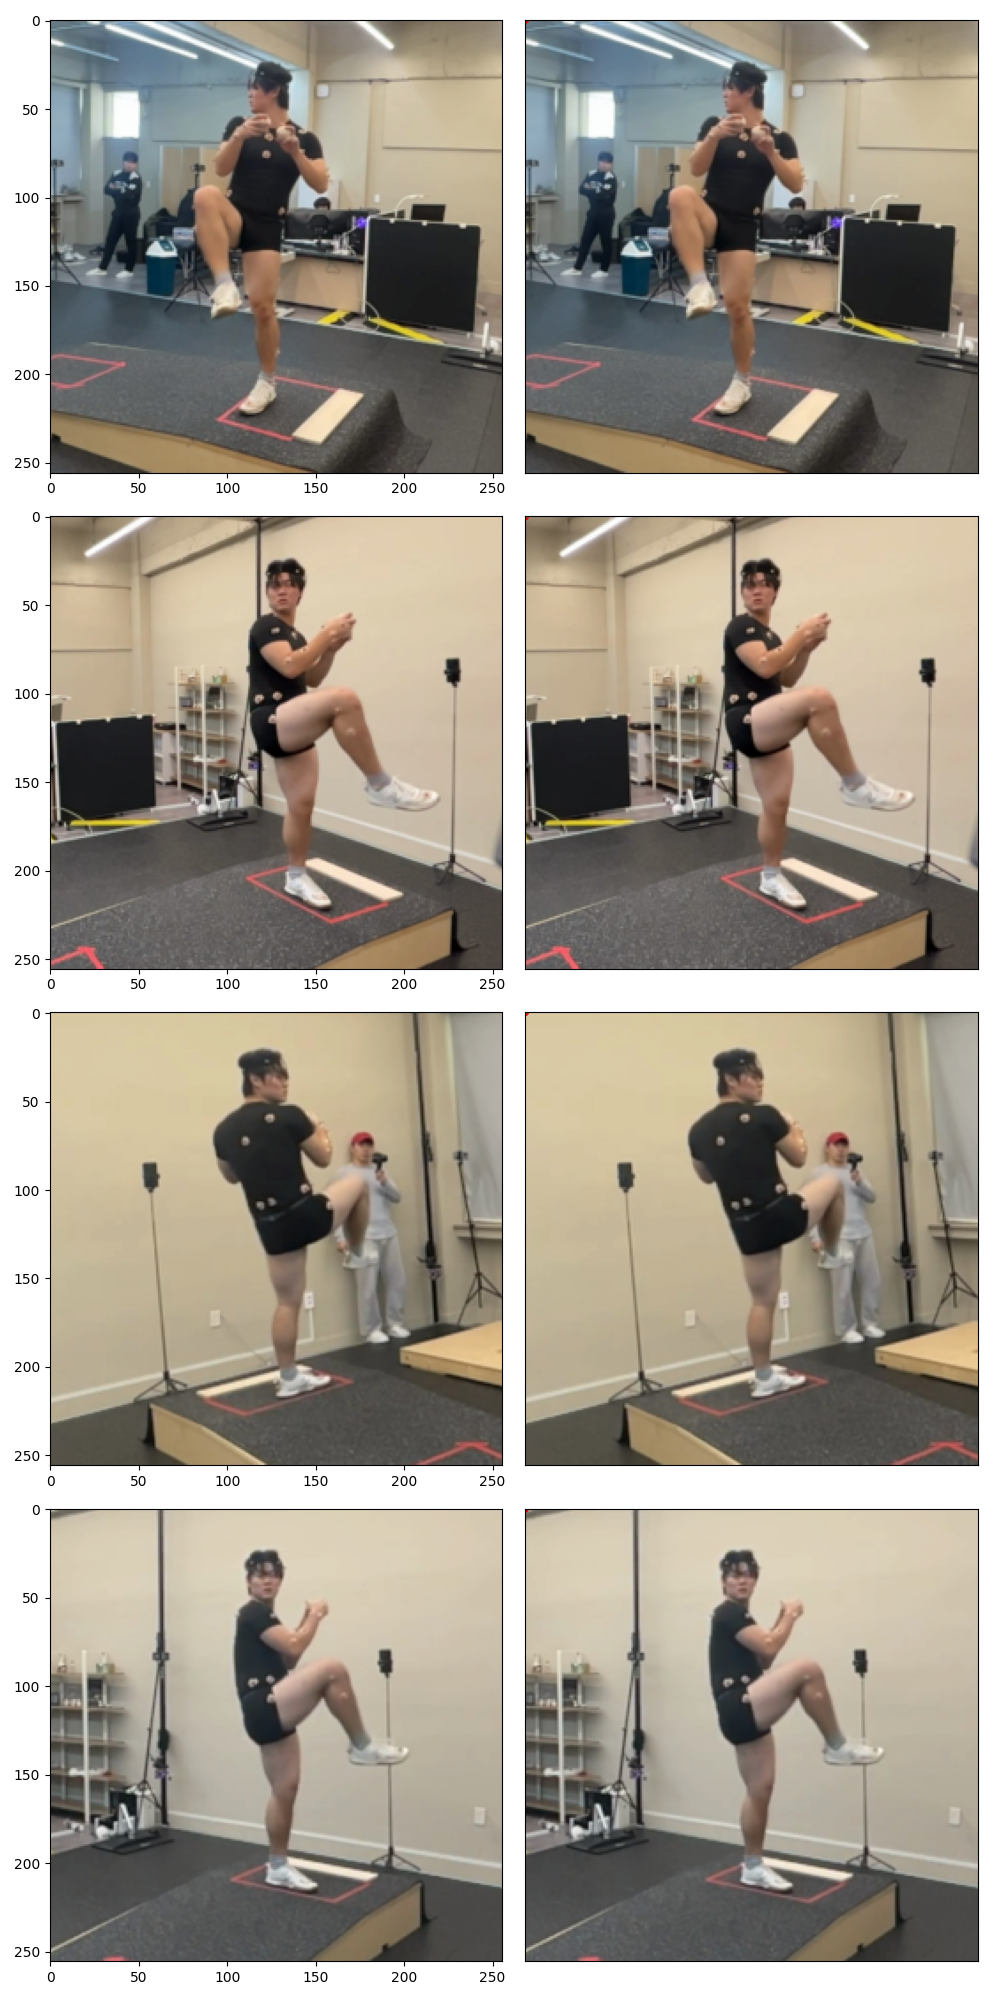
\includegraphics[width=0.5\textwidth]{data/uhmr_result/keypoints_2d_vis1.png}
\caption{U-HMR 2D keypoints 추정 결과: 4대 카메라에서의 관절점 검출. 각 뷰에서 투수의 포즈가 정확히 추정됨.}
\end{figure}

\begin{summary}
\textbf{U-HMR 핵심 성과}:
\begin{enumerate}[leftmargin=*]
  \item 4대 카메라 다시점 입력으로 \textbf{SMPL 메시 복원 성공}
  \item 투수의 wind-up 포즈가 정확히 재현 (들어올린 다리, 팔 위치)
  \item 각 뷰별 OBJ 메시 파일 출력
  \item 단일뷰 대비 \textbf{깊이 모호성 해소} --- 다시점 fusion의 효과
\end{enumerate}
\end{summary}


% ====================================================================
\chapter{SMPLest-X vs U-HMR 비교}
% ====================================================================

\begin{table}[H]
\centering
\caption{단일뷰 SMPLest-X vs 다시점 U-HMR 비교}
\renewcommand{\arraystretch}{1.4}
\begin{tabular}{p{4cm} p{5cm} p{5cm}}
\toprule
& \textbf{SMPLest-X} & \textbf{U-HMR} \\
\midrule
입력 & 단일 카메라 크롭 이미지 & 4대 카메라 동시 \\
모델 크기 & 0.69B (7.7GB) & ViT + Transformer decoder (8.2GB) \\
SMPL 버전 & SMPL-X (10,475 정점) & SMPL (6,890 정점) \\
출력 & 메시 좌표 (파라미터 아님) & SMPL 파라미터 + 메시 \\
깊이 추정 & 배경 context 의존 & 다시점 fusion \\
떨림 & 있음 (프레임 독립) & 적음 (다시점 일관성) \\
속도 & 4.5 fps (1대) & TBD (4대 동시) \\
GART 호환 & 역피팅 필요 & \textbf{직접 호환} \\
\bottomrule
\end{tabular}
\end{table}

\begin{keyidea}
\textbf{U-HMR이 GART 파이프라인에 더 적합}:
\begin{enumerate}[leftmargin=*]
  \item SMPL 파라미터를 직접 출력 $\rightarrow$ GART 입력으로 바로 사용 가능
  \item 다시점 fusion $\rightarrow$ 깊이 모호성 해소, 떨림 감소
  \item 단, 현재 4뷰 고정 --- 7뷰 확장 필요
\end{enumerate}
\end{keyidea}


% ====================================================================
\chapter{GART 설치 시도}
% ====================================================================

GART 설치를 시도했으나 \textbf{smplx 버전 호환성 문제}로 실행 실패:

\begin{enumerate}[leftmargin=*]
  \item \texttt{smplx.smplx} 모듈 경로 변경 $\rightarrow$ shim 패키지로 해결
  \item \texttt{SMPLOutput.J}, \texttt{SMPLOutput.A} 속성 미존재 $\rightarrow$ monkey patch 시도
  \item \texttt{.J}는 해결했으나 \texttt{.A} (bone transformation matrices)는 최신 smplx에서 반환하지 않음
  \item SMAL (동물 모델) 데이터 파일 미존재 $\rightarrow$ try-except로 우회
  \item SMPL 파라미터 float64/float32 타입 불일치 $\rightarrow$ 해결
\end{enumerate}

\begin{warningbox}
GART의 smplx 호환성 문제는 GART가 \textbf{smplx 0.1.13 이전 버전}의 내부 API에 의존하기 때문.
근본 해결: GART의 \texttt{templates.py}를 현재 smplx API에 맞게 리팩토링 필요.
또는 conda 환경을 분리하여 구버전 smplx 설치.
\end{warningbox}


% ====================================================================
\chapter{다음 단계}
% ====================================================================

\begin{enumerate}[leftmargin=*]
  \item \textbf{U-HMR 전체 시퀀스}: 1000프레임 $\times$ 4뷰 (또는 7뷰) 추론
  \item \textbf{U-HMR SMPL 파라미터 추출}: 프레임별 poses, betas, global\_orient, transl 저장
  \item \textbf{GART 호환성 해결}: smplx API 패치 또는 conda 환경 분리
  \item \textbf{GART 학습}: U-HMR SMPL 파라미터 + 다시점 이미지 $\rightarrow$ 3DGS 아바타
  \item \textbf{생체역학 분석}: SMPL2AddBiomechanics $\rightarrow$ OpenSim IK/ID
\end{enumerate}


\end{document}
